 \begin{frame}[allowframebreaks]{Nyquist-Shannon Grenze und Aliasing}
    \begin{itemize}
        \item Lt. Nyquist-Shannon-Theorem gilt:
    \end{itemize}
    \begin{equation}
        x[n] = \sin(2\pi \cdot f_0 \cdot n \cdot t_s) = \sin(2\pi \cdot (f_0 + kf_s) \cdot nt_s)
    \end{equation}
    Wobei: $k \in \mathbb{Z}$
    \begin{itemize}
        \item Daraus Folgt: Die Parameter $f_0$ und $(f_0 + kf_s)$ führen zum gleichen Amplitudenwert $\implies$ Nicht unterscheidbar
        \item Resultat: Mathematisch unendlich viele Aliase für jede Frequenz des Eingangssignals
    \end{itemize}
    \begin{figure}
        \centering
        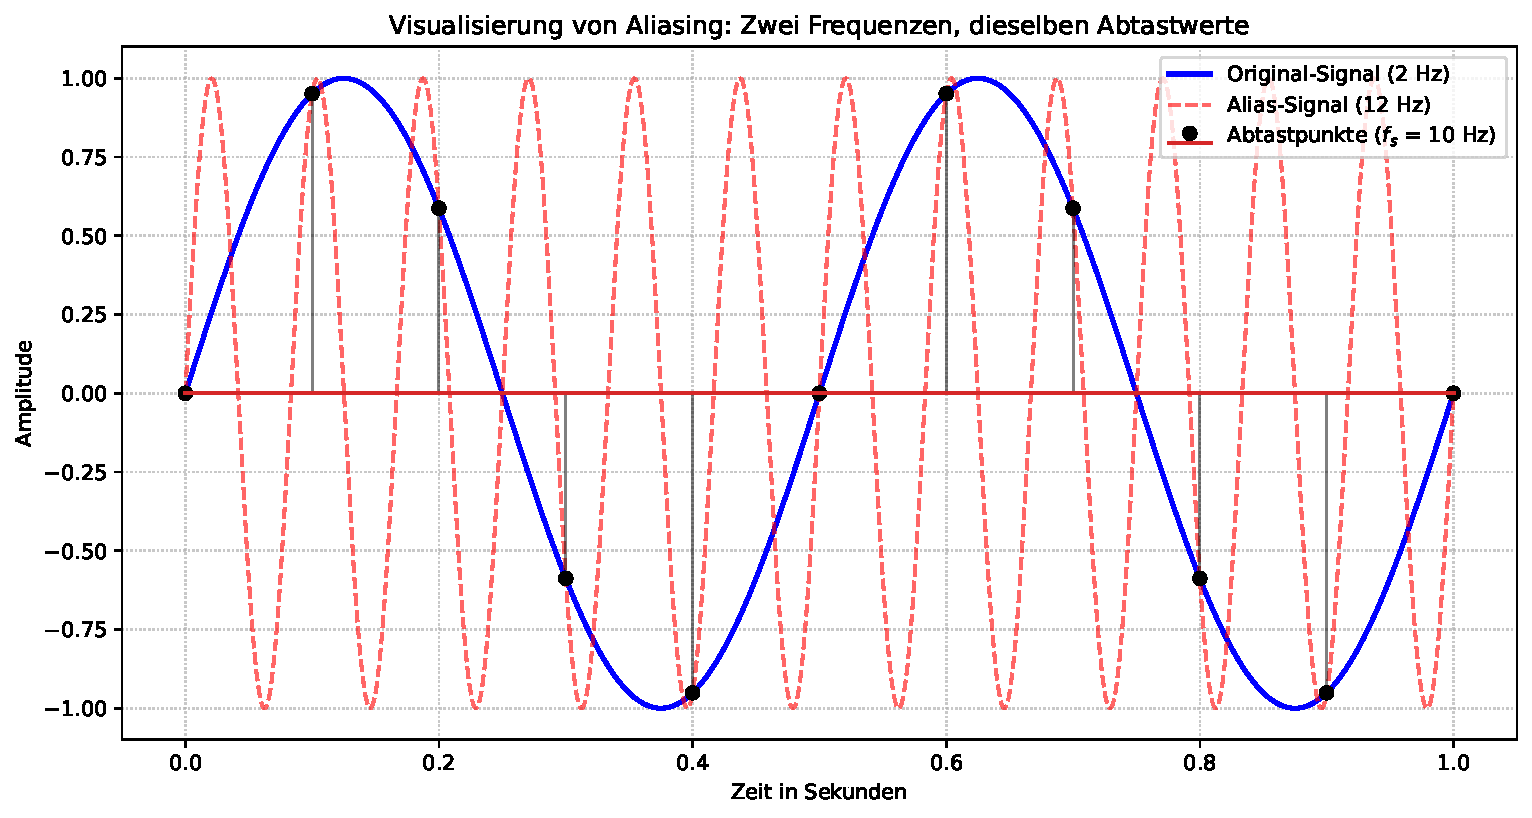
\includegraphics[width=0.6\textwidth]{Graphics/aliasing_vergleich.pdf}
        \caption{Für jedes Signal gibt es unendlich viele Interpretationsmöglichkeiten }
        \citeauthor{lyons2011}, \citeyear{lyons2011} \footcite[Kap. 2]{lyons2011}
    \end{figure}
 \end{frame}